 \section{Hardware}
%metatekst til hardware
<<<<<<< HEAD
Dette afsnit skal være med til at dokumentere hardwaren i systemet \textit{the cell collector}, derfor indeholder afsnittet fysiske dele og deres funktionalitet. De fysiske deles specifikationer er udybes og beskrevet i dette dokument. Der er begrundelser og argumenter for hvorfor de brugte komponenter er valgt.

\subsection{Læsevejledning til hardware}
%læsevejledning
Da dette afsnit er en udspecificering af hvilke specifikationer hardware komponenterne består af, ligger det sig tæt op af kravspecifikationen. Da det er kravene i kravspecfikationen, der ligger til grunde for de valgte hardware dele. I afsnittet findes der forskellige diagrammer der er med til at beskrive opbygningen, og kommunikationen af delene. Til hvert diagram vil der være en kort beskrivelse af hvad det beskriver. Hvert afsnit indeholder funktionalitet, specifikationer omkring det enkle komponent og begrundelser og argumentationer hvorfor det er valgt i den skrevne rækkefølge. AFsnitter kan godt læses i dele, men for den komplette forståelse bør afsnittet læses i rækkefølge. 

%Det gamle afsnit, måske skal det være i et leverandør afsnit 
% Dette afsnit indeholder den nødvendige viden hardware delene i systemet Denne blok beskriver forbindelserne mellem diverse hardware med et internal block definition diagram. Dette diagram er med til at sikre at delene kan kommunikere sammen, uden unødvendige adaptere og omformere. Yderligere er der beskrevet hvordan information søgning, og viden er fundet omkring komponenterne. Primær kan det siges at hardware delene er fundet på Ebay.com(kilder til de konkrete sider?(måske under hvert produkt?)), for at hold budgettet i bund. Den manglende datablade og lidt tvivlsomme kvalitet er accepteret, da dette projekt først og fremmest er  ”\textit{proof of concept}” projekt.
 
 
 
=======
 Dette afsnit indeholder alt omkring hardware delene, fra hvilke krav der er gået ud fra til hvad der er fundet frem til.  Afsnittet beskriver hvordan information søgning, og viden er fundet omkring komponenterne. Primært er hardware delene  fundet på Ebay.com (kilder til de konkrete sider?(måske under hvert produkt?)), for at holde budgettet nede. De manglende datablade og tvivlsomme kvalitet er accepteret, da dette projekt først og fremmest er  ”\textit{proof of concept}” projekt.

Nedenstående blokdiagrammer (figur: \ref{fig:bdd_Hardware} og figur: \ref{fig:ibd_Hardware}) beskriver hvilke hardware blokke systemet består af, samt forbindelserne mellem disse. Diagrammerne er med til at sikre at delene kan kommunikere sammen, uden unødvendige adaptere og omformere. 
>>>>>>> origin/master
 
 
 
 
 \newpage
\subsection{Block Definition Diagram} 
Et bdd diagram giver indblik i hardwarens overordnede struktur af systemet. Hver block er en del der indgår i systemet. Diagrammet er bygget hierarkisk system, hvor en blok kan indeholde flere blokke. blokkene består af en system blok \textit{the cell collector}, der indeholder tre elementære blokke, \textit{Arduino}, \textit{non electronic} og \textit{Camera}. Hvor \textit{Arduino} er den eneste der indeholder flere blokke, det beskriver hvilken hardware de overstående blokke kommuniker med.


\begin{figure}[H]
	\centering
	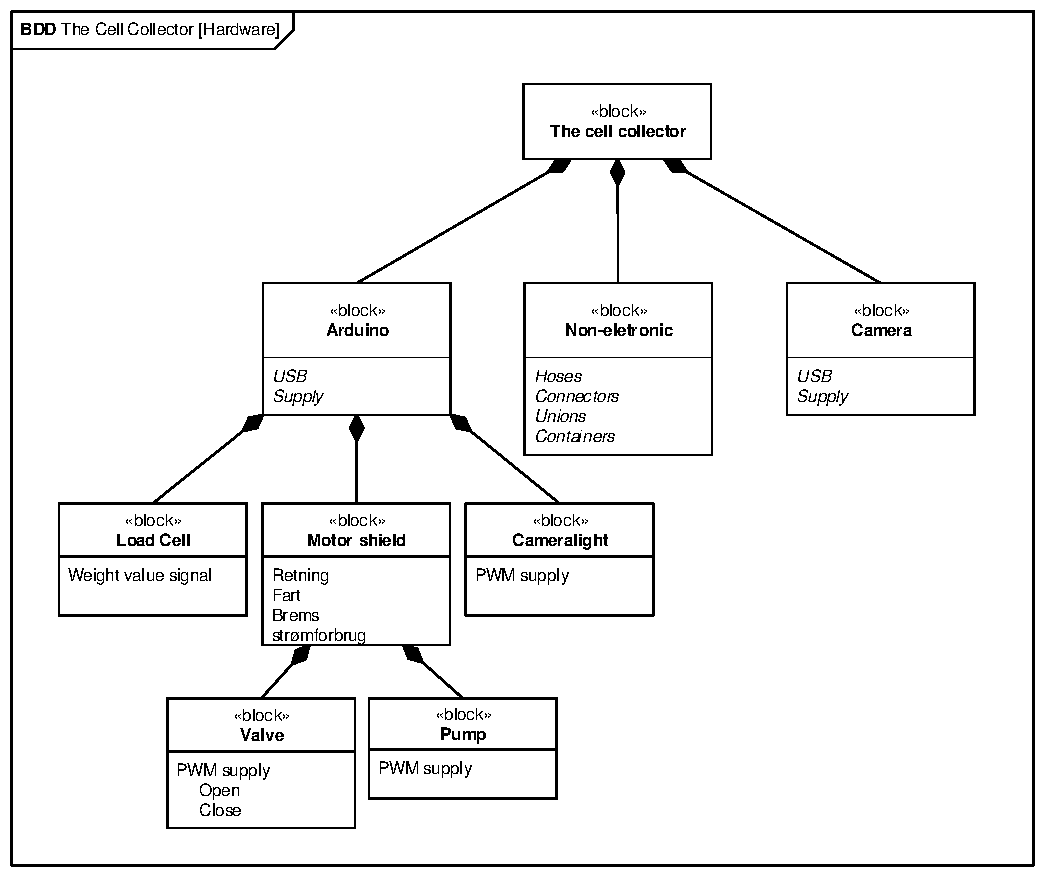
\includegraphics[width=1\textwidth]{pdf/BDD_Hardware_4315_cropped.pdf}
	\caption{BDD - Cell Collector [Hardware]}
	\label{fig:bdd_Hardware}
\end{figure}

<<<<<<< HEAD
\subsection{internal block Diagram} 
Et IBD diagram beskriver mere præcist, hvordan de forskellige komponenter med hinanden på. Det betyder at der er specialiseret indgangs- og udgangsporte, med de forskellige typer. Digrammet beskriver blandt andet, hvilken spænding delene arbejder under og hvilket signal der er brug for.
=======
\subsection{Internal block Diagram} 
>>>>>>> origin/master
\begin{figure}[H]
	\centering
	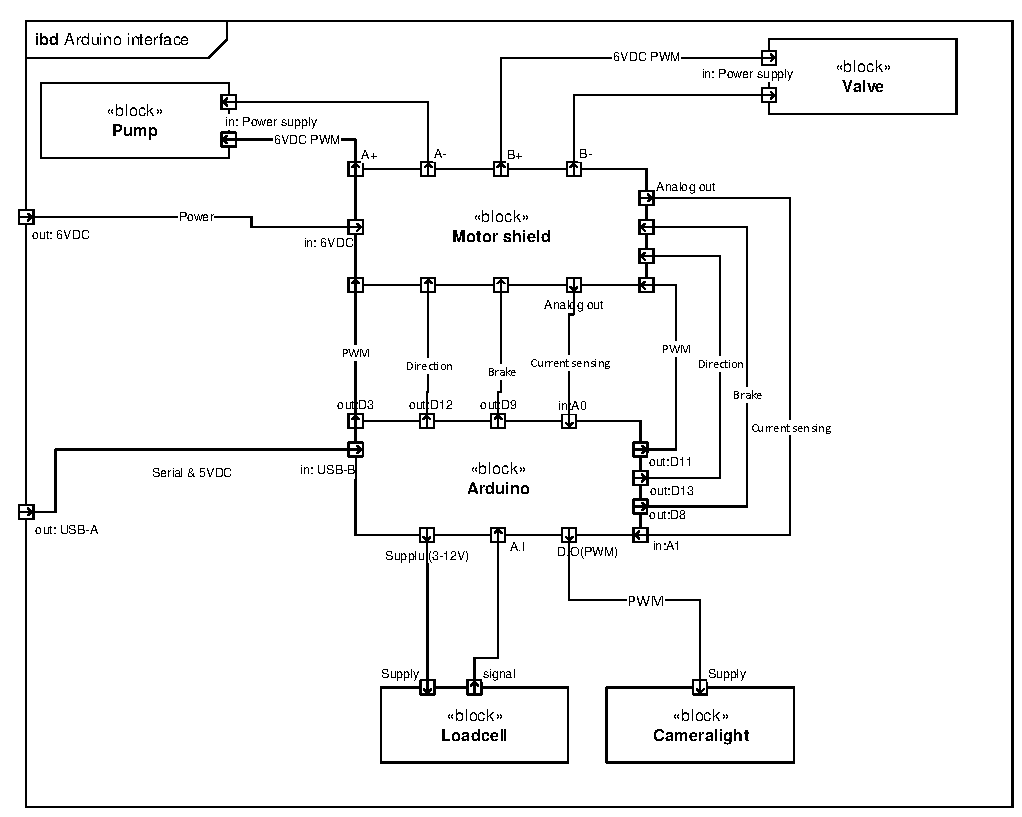
\includegraphics[width=1\textwidth]{pdf/IBD_Hardware(Arduino)_cropped.pdf}
	\caption{IBD - Cell Collector [Hardware]}
	\label{fig:ibd_Hardware}
\end{figure}



\subsection{Kamera}
Kameraet skal detektere de langerhanske øer, når de kommer forbi i slangen.  Da de langerhanske øer skiller sig ud ved at være mere lyse end resten af vævet, vil det være underordnet om kameraet er et farve kamera. Da systemet ikke skal operere under en stor hastighed er en standard frame rate valgt på 30 f/s. Kameraet opløsningen er valgt ud fra, at det skal kunne se de langerhanske øer med en størrelse på 100-300um. Til bestemmelse til dette er der brugt følgende formel:
 \fixme{Mangler formel}
For at kameraet har mulighed for, at se lidt flere detaljer og forhåbning om at det kan være tættere på end 10 cm, er det besluttet er et 2 megapixels kamera burde være passende.

\url{http://www.baslerweb.com/media/documents/BAS1408_White_paper_Camera_Selection_EN.pdf}


Da kameraet er en elementær del af systemet opsætning, blev det prioriteret, at købe det ved en mere pålidelig forhandler for at sikre en relativ god kvalitet, hvor prisen stadig lå inden for budgettet.  

Farnell
\url{http://dk.farnell.com/duratool/bw788/microscope-digital-usb-25x-200x/dp/2319420}
 
\subsection{Slanger}
Slangerne anvendes til at føre opløsningen med de langerhanske øer, i gennem systemet og bl.a. forbi kameraet. Da de største langerhanske øer, som systemet skal håndtere er 300um i diameter, er det valgt at slangerne skal have en indre diameter på 500um. Yderligere har et krav været at kameraet skal kunne se igennem slangerne, derfor er der tilkøbt et glasrør som kameraet kan se i gennem. 
%Grundet besvær med at finde en forhandler til de små mængder der skal anvendes til projektet, er der skabt kontakt til Mikrolab. Som har været en stor hjælp med at finde dele til slanger mm.

\subsection{Arduino}
Arduino er en open source platform til fremstilling af prototype print, som kan bruge til at styre forskellige systemer som dette. Arduino platformen er valgt da Matlab understøtter interaktion via en Support package. Boardet er brugt i et stort omfang omkring i verden. Derfor er det en platform der er nemt tilgængelig og forholdsvis prisvenlig, samt at der findes en stor mængde dokumentation omkring emnet. Da det som sagt er en open source platform, kan der købes forskellige versioner. 
Arduinoen skal bruges til at styre pumpen ved hjælp af ”mini motor drive shield”. Shielded anvendes for at være sikker på at der leveres effekt nok til pumpen. Yderligere har det den fordel at strømmen til pumpen kan måles og at den er galvanisk adskilt fra forsyningen til arduinoen. Dette er dog ikke arduinoen eneste opgave den skal blandt andet også styre ventilen til sortering og lyset til kameraet.

%Det er valgt at bruge en arduino som controller for at spare tid, i forhold til selv at lave et print med en microcontroller.
%Microcontrolleren der sidder på denne version er et gruppen har brugt, og arbejdet med til et tidligere projekt. Hvilket også betyder at den allerede er i gruppen beholdning af produkter.

\subsection{Ventil}
Ventilens funktion er at sorterer de langerhanske øer fra resten af opløsningen. Der findes utrolig mange typer af ventiler, med ret store prisforskelle. Ventilen er en vigtig del af systemets hardware, da det er dens ansvar at sortere de detekterede øer fra resten af væsken. Det er svært at finde ventiler med 500um studser. Det kan godt lade sig gøre at få adaptere så større ventiler kan bruges, men sporbarheden omkring hvor den enkelte ø befinder sig, bliver svært hvis kammeret pludseligt bliver stort. Dette er et stykke hardware, hvor der kan bruges meget tid og mange penge.
Kravene til ventilen er, at den skal være 3 vejs 1 tilgang og 2 udgange, yderligere skal studserne kunne tilpasses slange størrelsen, være til væske og have en lukke/åbne tid under 50ms.

\subsection{Pumpe}
Pumpen skal skabe det nødvendige flow i væsken fra det ene punkt til det andet. Flowet skal være lavt nok til at kameraet kan nå at detekterer en ø. Herfor er det et krav at pumpens flow hastighed er variabel, så flowet kan justeres. Der findes mange forskellige typer pumper til formålet, herunder stempel pumper, peristaltiske pumper og vakuum pumper. Der er bestilt en peristaltisk pumpe som virker ved at klemme på slangen og derved skabe et flow, det er dog uvist hvordan de langerhanske øer vil opfører sig ved sådan en pumpe. Der er også købt en vakuum pumpe, som muligvis kan sidde efter ventilen. Der skal dog stadig skabes et flow til de sorterede øers beholder, måske en kombination vil være det optimale. En modultest af de enkelte pumper skal afgøre hvilken løsning der er den mest optimale. 

\subsubsection{Vakuumpumper}
\url{ http://www.ebay.com/itm/281571300037}

\url{http://www.ebay.com/itm/161665897119?_trksid=p2054502.m570.l4467&_trkparms=gh1g%3DI161665897119.N19.S2.M-4218.R1.TR2}

\subsubsection{Peristaltiskepumper}

\url{http://www.ebay.com/itm/6V-Peristaltic-Pump-Dosing-Water-Pump-DC-Motor-Tube-For-Aquarium-Lab-Analytical-/131367703927?hash=item1e96201577}

%Ligesom ved ventilen er det også et produkt der kan få budgettet til at skride, derfor er der igen gået på kompromis og brug ebay forhandlere som leverandører.

\subsection{Beholdere}
Systemet består af tre beholdere der hver i især har sin egen funktion. Den første kaldes celleopløsningbeholderen, som skal indeholde den usorteret opløsning med de langerhanske øer. Beholder nummer to kaldes isolerede langerhanske øer beholderen, som er den beholder hvor de isolerede øer samles i. Den tredje beholder er waste beholderen, den skal have resten af opløsningen som ikke består af langerhanske øer. Størrelses kravene til beholderne er at opløsningsbeholderen skal mindst være 250ml, da det er den største mængde opløsning der vil blive brugt. Wastebeholderen skal således være dobbelt så stor, så der kan køres to sorterings cyklusser uden at skulle tømme beholderen i mellem. Den isolerede beholder, skal blot kunne rumme mængden af de isolerede øer. Da projektet som tidligere nævnt er et ”proof of concept” er den eneste beholder der er hentet informationer om opløsningsbeholderen. Den bør være støvtæt, uden at være lufttæt da der ellers vil dannes et vakuum i beholderen. Derudover vil det være en fordel hvis den er forholdsvis robust, så den kan køles ned osv. på et senere tidspunkt.

\subsection{Loadcell}
Loadcellen eller vægtcellen som det kan kaldes på dansk, skal bruges til at kontrollere om der er væske i celleopløsningsbeholderen. Den indkøbte vægtcellen kan veje op til 1 kg, hvilket fint dækker vægten for celleopløsningsbeholderen.

\url{http://www.ebay.com/itm/281311660424}

%Det vil sige hvs operatøren ikke har fyldt noget i beholderen, kan der gives en systembesked omkring dette. Det mest optimale er at der hele tiden er væske i slangerne i systemet, det er det vægtcellen skal hjælpe med.
